\documentclass[11pt]{article}
\usepackage[margin=1in]{geometry}
\usepackage{volfit_preamble}
\graphicspath{{figures/}}

\title{\textbf{Piecewise-Affine Local Volatility}\\[2pt]
\large Calibrating a Dupire surface from sparse quotes: model, PDE, gradients, and speed\\[2pt]
\normalsize Vol-Fitter Technical Notes, No.~04}
\author{Vol-Fitter}
\date{\today}

\begin{document}
\maketitle
% Auto-generated by gen_lv.py — do not edit.
\newcommand{\lvrtmaxerr}{0.6}
\newcommand{\lvrtwall}{0.94}
\newcommand{\lvrtnevals}{33}
\newcommand{\lvrtvtx}{28}
\newcommand{\lvrtsurfrms}{0.06}
\newcommand{\lvrtsurfmax}{0.25}
\newcommand{\lvgencommit}{77d43fb}
\newcommand{\lvgendate}{2026-07-11}
\newcommand{\lvspyrms}{2.4}
\newcommand{\lvnvdarms}{11.9}
\newcommand{\lvspyconv}{15.9}
\newcommand{\lvnvdaconv}{56.3}
\newcommand{\lvbenchtable}{\begin{tabular}{lrrr} \toprule Name & in-op RMS (bp) & converged RMS (bp) & worst expiry (bp)\\ \midrule SPY & 2.4 & 15.9 & 3.4\\ NVDA & 11.9 & 56.3 & 12.4\\ \bottomrule \end{tabular}}


\begin{abstract}
This note documents the Vol-Fitter's full local-volatility model: a continuous
piecewise-affine ($P_1$ finite-element) local-variance surface
$\nu_\theta(t,x)$, calibrated directly to sparse vanilla and variance-swap quotes
through the forward Dupire PDE as an implicit pricing map. Unlike the slice
models (Notes~01--03) this is a genuine two-dimensional local-volatility surface:
strict positivity of the nodal variances makes the implied prices butterfly- and
calendar-clean up to scheme noise, which the model \emph{measures} rather than
assumes. We derive the normalized forward Dupire equation, the $P_1$
parametrization and its positivity guarantee, the implicit-Euler discretization
and observation operator, the variance-swap log-contract replication and its
faster source-PDE alternative, and the calibration objective with its roughness,
convex-wing and front-tie regularizers. We then give the sensitivity PDE and the
adjoint gradient, and --- the engineering heart of the note --- the numerical
optimizations that took the cold fit from $\sim$\,86\,s to single-digit seconds:
a compiled vectorized-Thomas Dupire march ($\sim6.5\times$), a stall-based
early-stop, a parametric Dupire warm seed, and the matrix-free Gauss--Newton
solver that avoids the dense SVD. A synthetic round trip recovers a known surface
to \lvrtmaxerr\ vol bps, and the production fit on a static Bloomberg fixture
reaches \lvspyrms\ vol bps on SPY and \lvnvdarms\ on NVDA. The note closes with
the short-dated-fit fixes and the convex-wing regression that the benchmark
caught.
\end{abstract}

\tableofcontents
\newpage

%======================================================================
\section{The idea}
\label{sec:idea}

A slice model fits one expiry at a time and stitches expiries together with a
calendar constraint. A \emph{local-volatility} model does the opposite: it posits
a single function $\sigma_{\text{loc}}(t,S)$ such that, under
$\dd S_t=\sigma_{\text{loc}}(t,S_t)\,S_t\,\dd W_t$ (in forward-normalized units),
the model reproduces \emph{all} expiries and strikes at once. Dupire showed such a
function exists and is unique given an arbitrage-free price surface. The
Vol-Fitter follows the Andreasen--Huge philosophy: rather than \emph{differentiate}
a fitted price surface to extract $\sigma_{\text{loc}}$ (numerically explosive in
sparse data), it \emph{parametrizes} $\sigma_{\text{loc}}$ directly and prices
\emph{forward} through the Dupire PDE, calibrating the parameters to quotes.

\begin{heuristic}
Extracting local vol by the Dupire formula
$\sigma_{\text{loc}}^2=\partial_T C/(\tfrac12K^2\partial_{KK}C)$ divides two noisy
numerical derivatives of a sparse surface --- a recipe for garbage in the wings.
Calibrating local vol \emph{forward} instead never differentiates the data: it
asks ``what positive surface, run through the PDE, best reprices the quotes?''
Positivity of the surface is imposed on the \emph{parameters}, so every iterate is
arbitrage-clean by construction --- the same philosophy as LQD, one dimension up.
\end{heuristic}

%======================================================================
\section{The forward Dupire equation}
\label{sec:dupire}

Work in forward-normalized strike $x=K/F_T$ and let $c(T,x)$ be the normalized
call. Writing local variance $\nu(t,x)=\sigma_{\text{loc}}^2$, the forward Dupire
equation is
\begin{equation}
\boxed{\;\partial_T c(T,x)=\tfrac12\,\nu(T,x)\,x^2\,\partial_{xx}c(T,x),\qquad
c(0,x)=(1-x)^+.\;}
\label{eq:dupire}
\end{equation}
It is a forward parabolic PDE in $(T,x)$ with the call payoff as initial data.
Two facts make it the right object. First, $\partial_{xx}c\ge0$ is exactly the
butterfly (density) condition, and $\nu\ge0$ keeps the equation parabolic, so a
positive $\nu$ \emph{propagates} non-negativity of the density forward in
maturity. Second, monotonicity of $c$ in $T$ (the calendar condition) follows from
\eqref{eq:dupire} whenever $\nu\ge0$, since the right-hand side has the sign of
$\partial_{xx}c\ge0$. Thus a strictly positive local-variance surface is
\emph{structurally} free of both static arbitrages, up to the discretization noise
the model measures (\cref{sec:diagnostics}).

%======================================================================
\section{The piecewise-affine surface}
\label{sec:p1}

\subsection{Parametrization}

The local variance is a continuous piecewise-affine ($P_1$) function on a
tensor grid of $n_t\times n_x$ vertices $(\tau_i,\xi_j)$,
\begin{equation}
\nu_\theta(t,x)=\sum_{i,j}\theta_{ij}\,\phi_{ij}(t,x),
\label{eq:p1}
\end{equation}
where $\phi_{ij}$ are the bilinear (or barycentric/Delaunay) hat functions and
$\theta_{ij}=\nu(\tau_i,\xi_j)\ge0$ are the \emph{nodal local variances} --- the
calibration parameters. The flat vector is $\theta=\operatorname{vec}(\theta)$,
time-major.

\begin{proposition}[Nodal positivity $\Rightarrow$ surface positivity]
\label{prop:nodal}
A $P_1$ function is a convex combination of its vertex values on each cell. Hence
if $\theta_{ij}\ge0$ for all $i,j$, then $\nu_\theta(t,x)\ge0$ everywhere, and
$\nu_\theta>0$ if the nodal values are bounded below by a positive constant.
\end{proposition}

This is why the calibration enforces only \emph{box bounds} on $\theta$
(default local-variance bounds $[0.005,0.20]$, i.e.\ local vol in $[7\%,45\%]$):
positivity of the whole surface reduces to positivity of finitely many numbers.
Beyond the lowest strike vertex the surface extrapolates the local variance
\emph{linearly} with a slope set by the first interior cell
(\texttt{left\_extrap\_a}; Note~09), rising toward $x\to0$; the right wing is
flat-clamped.

\subsection{Grid design}

The vertex grid is delta-spaced in strike and floored per expiry so that even a
narrow short-dated smile lands enough vertices on its curvature
(\texttt{gridXNodes}, \texttt{gridXMinPerExpiry}; \cref{sec:short}). The time
vertices (\texttt{gridTNodes}) carry the term structure. The grid is deliberately
modest --- a dozen strike vertices, ten in time --- because each vertex is a free
parameter and the PDE solve cost scales with the grid; the regularizer
(\cref{sec:objective}) supplies the smoothness that a coarse grid would otherwise
lack.

%======================================================================
\section{The pricing map}
\label{sec:pricing}

\subsection{Discretization}

The PDE \eqref{eq:dupire} is solved on a uniform spatial grid $x_g$ (default
$\sim$\,$1201$ nodes spanning several standard deviations, \texttt{DEFAULT\_N\_K})
by fully implicit (backward) Euler in maturity with step $\le$ \texttt{DEFAULT\_DT\_MAX}
$=1/400$, optionally Rannacher-started (a few implicit quarter-steps before
Crank--Nicolson). Each step solves a tridiagonal $M$-matrix system
\begin{equation}
(I-\Delta T\,A_n)\,U^{n+1}=U^{n},
\label{eq:implicit}
\end{equation}
where $A_n$ encodes $\tfrac12\nu\,x^2\partial_{xx}$ at step $n$. The matrix is an
$M$-matrix (diagonally dominant, non-positive off-diagonals), so the scheme is
unconditionally stable and monotone --- it cannot create spurious negative
densities. The observation operator reads the normalized call at each quote's
$(T,x)$ off the solution by interpolation.

\subsection{No-arbitrage diagnostics}
\label{sec:diagnostics}

Because the surface is only \emph{up to scheme noise} arbitrage-free, the model
measures the residual: a butterfly tolerance on $\partial_{xx}c$ and a calendar
tolerance on $\partial_T c$ (both $10^{-8}$). The model is gated behind these
diagnostics rather than assuming cleanliness --- a deliberate design choice.

%======================================================================
\section{Variance swaps}
\label{sec:varswap}

A variance-swap quote is the fair strike of realized variance, which for a
diffusion equals the expected total variance to $T$. Two pricers are available.
The \emph{static} method uses the log-contract replication
\begin{equation}
I(T)=2\!\int_0^1\frac{P(T,x)}{x^2}\,\dd x+2\!\int_1^\infty\frac{C(T,x)}{x^2}\,\dd x,
\label{eq:logcontract}
\end{equation}
a trapezoid over the priced surface (half-width and node count
\texttt{VS\_HALF\_WIDTH}, \texttt{VS\_POINTS}). The faster \emph{source-PDE}
method (default-off, gated by \texttt{varSwapMethod}) solves one backward source
PDE $\partial_t g+\tfrac12\nu x^2\partial_{xx}g+\nu=0$, $g(T,\cdot)=0$, and reads
$I(T)=g(0,1)$ --- with analytic sensitivities $\partial I/\partial\theta$ from the
same multi-RHS machinery, and without the $x_{\max}$-dependence of the
replication tail. Note~08 develops both in full.

%======================================================================
\section{The calibration objective}
\label{sec:objective}

The fit minimizes a stacked least-squares residual over $\theta$,
\begin{equation}
\min_{\theta\in[\nu_{\mathrm{lo}},\nu_{\mathrm{hi}}]}\ \tfrac12\Big(
\underbrace{\|r_{\text{opt}}\|^2}_{\text{quotes}}
+\underbrace{\|r_{\text{vs}}\|^2}_{\text{var-swaps}}
+\underbrace{\lambda\|L(\theta-\theta_{\text{ref}})\|^2}_{\text{roughness}}
+\underbrace{w_{\text{cvx}}\|r_{\text{cvx}}\|^2}_{\text{convex wing}}
+\underbrace{w_{\text{ft}}\|r_{\text{ft}}\|^2}_{\text{front tie}}\Big),
\label{eq:lv_objective}
\end{equation}
with the blocks:
\begin{itemize}[leftmargin=1.4em]
\item \textbf{Option residuals} $r_{\text{opt},q}=(P_q(\theta)-y_q)/\eta_q$ in
vega-normalized forward-call price units (mid), or the bid--ask/haircut band hinge
with a small mid anchor when band edges are present (Note~07).
\item \textbf{Var-swap residuals} $r_{\text{vs}}=(I(\theta)-z)/\zeta$ (Note~08).
\item \textbf{Roughness} $\sqrt\lambda\,L(\theta-\theta_{\text{ref}})$ with $L$ the
spacing-aware second-difference operator and $\theta_{\text{ref}}$ a reference
surface; the time-vs-strike balance is \texttt{gridRegRho}. This is the smoothness
that lets a coarse grid generalize.
\item \textbf{Convex wing} hinge: a one-sided penalty enforcing local convexity of
the wing, confined to vertices \emph{below the deepest quote} (the extrapolation
tail only --- see \cref{sec:convexbug}).
\item \textbf{Front tie}: a light penalty tying the front-end vertices to the ATM
level where the shortest expiry has little strike coverage.
\end{itemize}

%======================================================================
\section{Sensitivities and the adjoint}
\label{sec:sens}

\subsection{The sensitivity PDE}

Each parameter $\theta_\ell$ enters \eqref{eq:dupire} linearly through $\nu_\theta$,
so the price sensitivity $s_\ell=\partial c/\partial\theta_\ell$ obeys the same
parabolic PDE with a \emph{source}:
\begin{equation}
\partial_T s_\ell=\tfrac12\nu_\theta x^2\partial_{xx}s_\ell
+\tfrac12\phi_\ell\,x^2\partial_{xx}c,\qquad s_\ell(0,\cdot)=0.
\label{eq:senspde}
\end{equation}
Discretized, every $s_\ell$ shares the \emph{same} tridiagonal factor as the value
solve \eqref{eq:implicit}, differing only in the source --- so the Jacobian columns
are a single multi-RHS back-substitution against one factorization. This is the
forward-sensitivity route, $O(N_t N_x m)$ for $m$ active parameters.

\subsection{The adjoint gradient}

When only the \emph{gradient} of the scalar objective is needed (not the full
Jacobian), the discrete adjoint computes it in one forward value solve plus one
backward adjoint sweep, $O(N_t N_x)$ \emph{independent of $m$}. The Vol-Fitter
uses the forward sensitivities for the Gauss--Newton Jacobian (it needs the
columns) and keeps the adjoint as the route for very large vertex counts.

%======================================================================
\section{Solvers and the speed story}
\label{sec:solvers}

The cold fit of \eqref{eq:lv_objective} was, at $\sim$\,533 vertices, an
$\sim$\,86\,second affair hitting the $200$-evaluation cap --- the single heaviest
computation in the app. Driving it down is most of the engineering in this model,
and the lessons are worth stating because several plausible ideas \emph{failed}.

\subsection{Where the time goes}

On a cold fit the cost splits roughly as: optimizer linear algebra / dense SVD
$\sim52\%$, PDE sensitivity march $\sim32\%$, Jacobian assembly $\sim14\%$, value
solve $\sim2\%$. No single per-evaluation lever moves the total, because the cost
is distributed --- which is why four separate ``faster per evaluation'' attempts
(coarse grid, first Numba try, Rannacher, and the first matrix-free GN) each won
only $\sim1.1$--$1.2\times$ and were shelved.

\subsection{What worked}

\begin{perfbox}
The cold fit is now $\sim3$--$6\times$ faster than the original banded baseline
(scaling with grid size); recalibrations are near-instant via warm start. The
levers, in order of impact:
\begin{enumerate}[leftmargin=1.5em]
\item \textbf{Stall-based early-stop.} Track the option-block misfit and stop at
the best iterate once it stalls. Because fewer evaluations multiply march,
assembly \emph{and} optimizer together, this scales the \emph{whole} fit:
measured $1.45\times$ (SPY) to $3.3\times$ (NVDA), at $+0.1$--$0.25$ vol bp.
\item \textbf{Compiled vectorized-Thomas march.} A \texttt{@njit} no-pivot Thomas
solver with the sensitivity columns as the contiguous SIMD inner loop and a fused
source: $\sim6.5\times$ the LAPACK banded march, numerically exact to $\sim10^{-15}$.
The first Numba attempt (column-outer scalar Thomas) won only $1.2\times$ --- the
real lever was the loop order.
\item \textbf{Matrix-free Gauss--Newton.} The default solver avoids
\texttt{trf}'s dense SVD (52\% of an evaluation) by solving the GN step with
preconditioned LSMR on matrix-free $Jv$/$J^{\mathsf T}w$ products. Once the march
is cheap, the no-SVD evaluations win: $\sim1.3$--$1.65\times$ over TRF. Gated to
the smooth mid-fit target.
\item \textbf{Parametric Dupire warm seed.} Seed $\theta$ from the parametric
surface's local variance ($\sim1.3$--$1.8\times$ on cold fits) and from the
previous surface on recalibration ($\sim38\times$).
\end{enumerate}
The order-of-magnitude wins are spent; remaining levers are incremental.
\end{perfbox}

\begin{caution}
Removing the dense SVD made fits \emph{slower} at $\le440$ vertices, because there
the bottleneck is the PDE march, not the SVD --- the SVD wall is a $\gtrsim1000$-vertex
(future non-tensor ``bowtie'' grid) phenomenon. The clean synthetic benchmark
(zero residual, in bounds) hid this: GN converged in $8$ evaluations there but did
\emph{not} converge within the cap on stiff real data. The honest lesson: measure
on real chains, and distrust a synthetic-only speed-up.
\end{caution}

%======================================================================
\section{Short-dated calibration}
\label{sec:short}

A genuine one-week smile fit \emph{catastrophically} (108 vol bp RMS vs the
parametric $\sim47$) while normal expiries fit well. A measure-first diagnosis
(per-expiry side-channel counting in-range vertices, vega flooring and PDE steps)
ruled out the usual suspects --- vega floor, time steps, local-vol cap, prior
leakage --- and isolated \emph{strike under-resolution}: the delta strike axis is
sized to the \emph{longest} expiry and clipped to the global range, so a narrow
short smile landed only $\sim3$ vertices on its sharpest curvature. Two fixes:
\begin{enumerate}[leftmargin=1.5em]
\item \textbf{Per-expiry coverage floor} (\texttt{gridXMinPerExpiry}, default $8$):
after the delta axis is built, split the widest in-range gaps until each expiry
has at least $m_{\min}$ vertices inside \emph{its own} traded range --- adding nodes
only to under-covered short fronts.
\item \textbf{Short-expiry-aware PDE step}: refine the shared PDE $x$-step to
$0.3\times$ the smallest ATM $\sigma\sqrt\tau$, snapped so $x=1$ stays a node,
clamped to $[1/400,\,0.01]$. Normal surfaces stay on $0.01$ (byte-identical).
\end{enumerate}
The one-week fit fell from $108\to23.5$ vol bp (now \emph{better} than the
parametric), with the long expiries byte-identical.

\subsection{The convex-wing regression}
\label{sec:convexbug}

The benchmark also caught a subtler bug. The convex-wing constraint originally
selected \emph{every} vertex in the deep wing regardless of data; at a user's
saved $\texttt{gridXNodes}=20$ it stacked convexity penalties onto densely-quoted
put strikes and forced the \emph{wrong} wing on low-vol SPY (NVDA's naturally
convex wing had hidden it). The fix confines \texttt{convex\_cols} to vertices
\emph{below the deepest quote} --- the extrapolation tail only. SPY went
$25.7\to2.6$ vol bp. The lesson echoes Note~09: a shape constraint must not be
imposed where the data already speaks.

%======================================================================
\section{Worked examples}
\label{sec:examples}

\subsection{Synthetic round trip}

A known skewed local-variance surface is priced through the forward PDE, quotes
are generated at four expiries, and the surface is recovered from a \emph{flat}
seed by the production calibrator. \Cref{fig:lv} shows the recovered surface and
the implied-vol fit: the calibrator recovers the truth to a maximum of
\lvrtmaxerr\ vol bps in \lvrtnevals\ evaluations (\lvrtwall\,s wall,
\lvrtvtx\ vertices), with the skew (higher local vol at low strike) faithfully
reconstructed.

\begin{figure}[H]
\centering
\begin{minipage}{0.52\textwidth}\centering
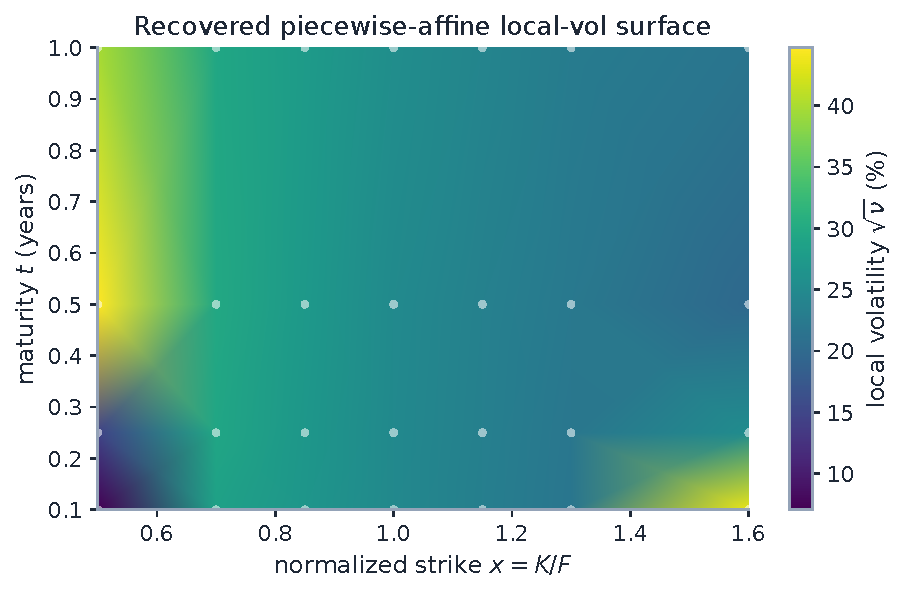
\includegraphics[width=\textwidth]{fig_lv_surface.pdf}\\[1pt]
{\footnotesize (a) recovered local-vol surface}
\end{minipage}\hfill
\begin{minipage}{0.45\textwidth}\centering
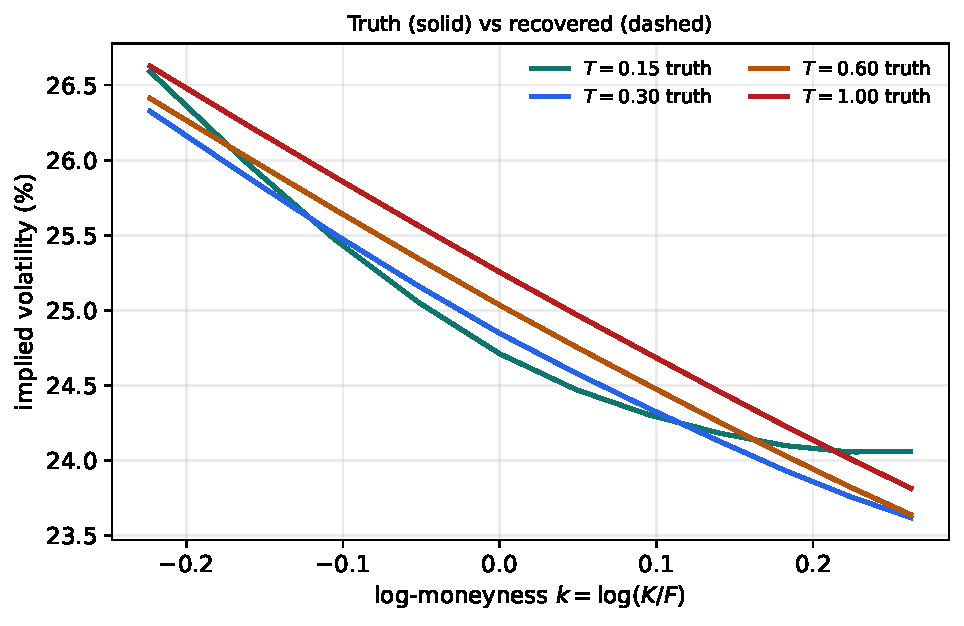
\includegraphics[width=\textwidth]{fig_lv_fit.pdf}\\[1pt]
{\footnotesize (b) IV fit, truth vs recovered}
\end{minipage}
\caption{Synthetic round trip through the real calibrator: the skewed surface is
recovered to \lvrtmaxerr\ vol bps from a flat seed.}
\label{fig:lv}
\end{figure}

\subsection{The Bloomberg benchmark}

On the static Bloomberg fixture the production fit reaches the quality in
\cref{tab:bench} and \cref{fig:rms}: \lvspyrms\ vol bps surface RMS on SPY and
\lvnvdarms\ on NVDA, with no node at a bound on the easy expiries. The harder
NVDA short-dated expiries carry the larger error --- the regime
\cref{sec:short} addresses.

\begin{table}[H]
\centering
\caption{Production local-vol fit on the Bloomberg fixture (fresh run).}
\label{tab:bench}
\lvbenchtable
\end{table}

\begin{figure}[H]
\centering
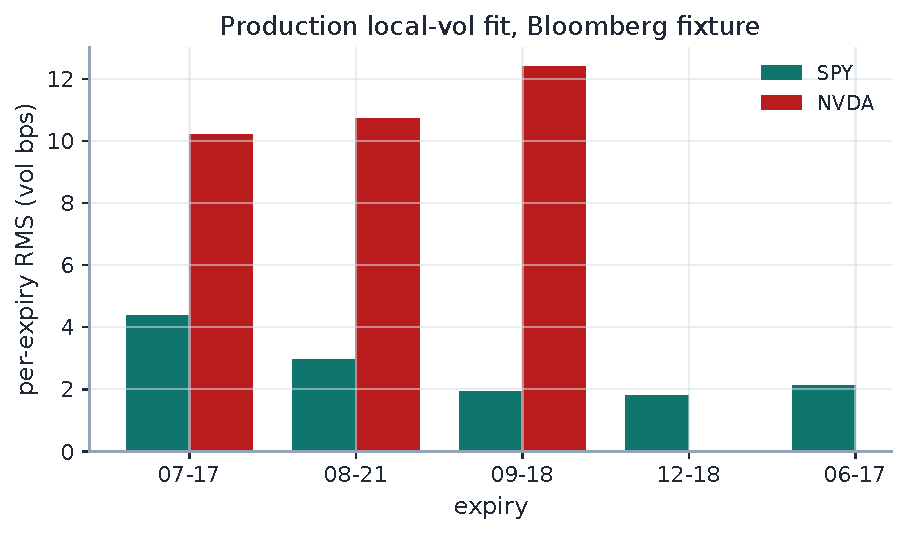
\includegraphics[width=0.74\textwidth]{fig_lv_rms.pdf}
\caption{Per-expiry weighted RMS for SPY and NVDA on the fixture.}
\label{fig:rms}
\end{figure}

%======================================================================
\section{What is original, and limitations}
\label{sec:original}

The $P_1$-positivity guarantee and the forward-calibration philosophy are
Andreasen--Huge; the contributions here are engineering depth. The
\emph{vectorized-Thomas Numba march} (loop order as the lever, $6.5\times$), the
\emph{stall early-stop} that scales the whole fit, the \emph{matrix-free GN}
correctly scoped to where the SVD actually dominates, the \emph{source-PDE
var-swap} with analytic sensitivities, and the \emph{measure-first} short-dated
diagnosis are each non-obvious and were validated against a real benchmark that
twice caught regressions a synthetic would have missed. Limitations: the model is
a pure diffusion (no jumps), so a true short-dated event spike is only
approximated; the tensor grid wastes vertices in the corners (the future
non-tensor bowtie grid is where GN's no-SVD advantage would finally dominate); and
the fit, though much faster, remains the heaviest single computation in the app.

\appendix
%======================================================================
\section{Hyperparameter atlas}
\label{app:atlas}

\begin{longtable}{p{0.26\textwidth}p{0.14\textwidth}p{0.52\textwidth}}
\caption{Local-volatility hyperparameters.}\label{tab:atlas}\\
\toprule Knob & Default & Role\\ \midrule
\endfirsthead \toprule Knob & Default & Role\\ \midrule \endhead
\multicolumn{3}{l}{\emph{Surfaced (OptionsSettings)}}\\ \midrule
\texttt{gridXNodes} & $12$ & Strike vertices of the variance surface.\\
\texttt{gridXMinPerExpiry} & $8$ & Min in-range strike vertices per expiry (\cref{sec:short}).\\
\texttt{gridTNodes} & $10$ & Maturity vertices.\\
\texttt{gridRegLambda} $\lambda$ & $10^{-2}$ & Roughness penalty strength.\\
\texttt{gridRegRho} $\rho$ & $1.0$ & Time-vs-strike roughness balance.\\
\texttt{convexWingWeight} & $10^{3}$ & Convex-wing hinge weight (tail only).\\
\texttt{frontTieWeight} & $10^{-2}$ & Front-end tie-to-ATM weight.\\
\texttt{lvVolCapMult} & $3.0$ & Local-vol cap as a multiple of max implied vol.\\
\texttt{leftWingSlopeMult} & $1.5$ & Left local-variance extrapolation slope multiple.\\
\texttt{varSwapMethod} & \texttt{static} & Var-swap pricer: replication or source-PDE.\\
\texttt{lvSolver} & \texttt{gn} & Gauss--Newton (default) or \texttt{trf}.\\
\texttt{lvFastKernel} & \texttt{true} & Numba vectorized-Thomas march.\\
\texttt{lvEarlyStop} & \texttt{true} & Stall-based early stop.\\
\texttt{timeScheme} & \texttt{implicit} & Implicit Euler or Rannacher/CN.\\
\midrule
\multicolumn{3}{l}{\emph{Hidden (PDE / solver)}}\\ \midrule
\texttt{DEFAULT\_N\_K} & $1201$ & PDE spatial nodes.\\
\texttt{DEFAULT\_DT\_MAX} & $1/400$ & PDE max time step.\\
\texttt{N\_RANNACHER} & $4$ & Rannacher start quarter-steps.\\
\texttt{SPAN\_SD} / \texttt{SPAN\_MIN} & $7.5$ / $0.6$ & PDE grid span (sd / floor).\\
\texttt{VAR\_FLOOR} & $10^{-6}$ & Dupire local-variance floor.\\
variance bounds & $[0.005,0.20]$ & Nodal local-variance box (vol $[7\%,45\%]$).\\
\texttt{x\_scale} & \texttt{jac} & Optimizer column scaling.\\
\texttt{xtol/ftol/gtol} & $10^{-8}$ & Optimizer tolerances.\\
\texttt{max\_nfev} & $200$ & Evaluation cap.\\
\texttt{stall\_window/rtol} & $12$--$18$ / $\sim3\text{--}5\!\times\!10^{-3}$ & Early-stop window/tolerance.\\
\bottomrule
\end{longtable}

%======================================================================
\section{Performance notes}
\label{app:perf}

\begin{enumerate}[leftmargin=1.6em]
\item \textbf{Numba march} (\texttt{lvFastKernel}). No-pivot factor-once Thomas
with the $m$ sensitivity columns as the contiguous inner SIMD loop and fused
source: $6.1$--$6.9\times$ vs LAPACK \texttt{dgbsv}, exact to $\sim10^{-15}$.
Graceful banded fallback if Numba is absent.
\item \textbf{Early stop} (\texttt{lvEarlyStop}). Best-iterate stop on option-block
stall; scales the whole fit, $1.45\times$ (SPY) to $3.3\times$ (NVDA), $+0.1$--$0.25$
vol bp. \texttt{stall\_window}$=0$ is byte-identical.
\item \textbf{Matrix-free GN} (\texttt{lvSolver=gn}). Preconditioned LSMR on
$Jv$/$J^{\mathsf T}w$; avoids the dense SVD. $1.3$--$1.65\times$ over TRF at
tensor-grid sizes; gated to the smooth mid target.
\item \textbf{Warm starts.} Previous-surface seed ($\sim38\times$ recal) and
parametric Dupire cold seed ($1.3$--$1.8\times$).
\item \textbf{Shelved (documented):} coarse grid (biases $\theta$), first Numba
attempt (wrong loop order), Rannacher ($1.1\times$ + arb risk), GN for the
non-smooth band objective, thread/process parallelism (GIL). Four distributed-cost
dead-ends confirming the cost is spread, not localized.
\end{enumerate}

\begin{thebibliography}{9}
\bibitem{Dupire1994} B.~Dupire. Pricing with a smile. \emph{Risk}, 7(1):18--20, 1994.
\bibitem{AndreasenHuge2011} J.~Andreasen and B.~Huge. Volatility interpolation.
\emph{Risk}, March 2011.
\bibitem{Gatheral2006} J.~Gatheral. \emph{The Volatility Surface}. Wiley, 2006.
\bibitem{GilesCarter2006} M.~Giles and R.~Carter. Convergence analysis of
Crank--Nicolson and Rannacher time-marching. \emph{J.\ Comput.\ Finance}, 9(4), 2006.
\end{thebibliography}

\end{document}
